\chapter{Pattern recognition}
In this chapter, we describe several classes of algorithms for pattern recognition. In the first part, we review some of the algorithms, namely the \emph{Normalized cross-correlation}, \emph{Shape matching and object recognition using shape contexts} and \emph{Matching of Shapes Using Dynamic Programming}. The second section is devoted to the \emph{Artificial neural networks} in the context of pattern recognition, which are later used for the implementation of thesis goal.

Pattern recognition problem is a broad term for classification problems that are based on the similarity of the features of classified objects. Precise mathematical definition can be found in the work of \citet{formalMethods}. We will focus more on the shape recognition problems category, which is a form of pattern recognition. A shape can be typically defined as an equivalence class under the group of transformations, and the problem is then to algorithmically approximate the human-like visual pattern recognition. 
We define an image as a two-dimensional grid of pixels with values from the range $[0,1]$ and we define the shape as a group of image instances where a human sees the same shape.

\section{Algorithms classification}
There are many of algorithms on for pattern recognition that can be categorized based on different criteria. \citet{imageRecognition} categorize the algorithms into following approach-based classes:
\begin{description}
\item [Statistical approach] Algorithms in this category are based on the underlaying probability model. The shape class is determined by the features that can be automatically extracted from its members and the probability distributions of the shape belonging to each class. An example of such algorithm is the naive Bayess classifier.

\item [Nonmetric approach] This class contains decision tress, syntactic methods, and rule-based classifiers. The idea of these algorithms is that each shape can be decomposed into the simplest sub-patterns called primitives. These primitives are then viewed as a language and the shape class as a set of rules, from which the shape can be derived. However, the inference of the grammar rules from the training data and the detection of the primitives are difficult problems.

\item [Cognitive approach] Neural networks and support vector machines belong to this class. Neural networks are inspired by biological neural structures. They can be described as massively parallel computation systems that can learn complex input-output relationships.

At the same time, \cite{imageRecognition} remark:
\begin{quotation} However, in spite of the seemingly different underlying principles, most of the neural network models are implicitly similar to statistical pattern recognition methods. \end{quotation}

\end{description}

\cite{skeletonMatching} proposes in the work different classification based on the creation process of the classifier. The algorithms are divided into learning-based approaches and template-based approaches. In the learning-based approaches, pattern classifiers are obtained through training on pre-classified samples. In the template based approaches, patterns are described by templates and the recognition problem is transformed into searching for the best matching template for a given input image.

Another classification proposed by \citet{distanceTransform} divides the algorithms into three classes based on the level of preprocessing:
\begin{itemize}
\item Algorithms that use pixel values directly, e.g. correlation-based methods. Example from this category is the normalized cross-correlation, described in \cref{normalizedCC}.
\item Algorithms that use low-level features such as edges and corners, e.g. distance transform method, described in \citet{distanceTransform}.
\item Algorithms that use high-level features such as identified objects or relation between the features, e.g. graph-theoretic-methods \cite{graph}.
\end{itemize}

Given the amount of algorithms to choose from, we have decided to review only a few of them, namely the normalized cross-correlation, shape contexts object matching and matching of shapes using dynamic programming, and the general approach of using the neural networks, which we use in our algorithm implementation.

\section{Normalized cross-correlation}
\label{normalizedCC}
Following description is based on the work of \cite{crossCorrLewis}.
Cross-correlation is a method to measure the similarity between a template and a given area of an image, both in the form of a grid of pixel values. The term cross-correlation itself means a difference between two signals. It is one of the oldest approaches to pattern and feature recognition and extraction, and still serves as a base for more complex algorithms.

It works by computing the distance between an image and the searched template. We can compute an Euclidean distance of a image f and a template t, where pattern is on a position $(u\,v)$, by comparing corresponding pixels of the image at $(x\,y)$ and the template shifted to $(x-u\,y-v)$.
\[d_{f,t}^{2}(u,v)=\sum_{x,y} [ f(x,y) - t(x-u, y-v) ]^{2}\]
When expanded, it gives us three terms. One of them is the cross correlation term $c(u,v)$.
\begin{align*}
d_{f,t}^{2}(u,v)=&\sum_{x,y} f(x,y)^{2} - 2c(u,v) + \sum_{x,y} t(x-u, y-v)^2 \\
c(u,v)=&\sum_{x,y} f(x,y) * t(x-u, y-v).
\end{align*}

Other two terms express the energy (brightness) of the template and the image, respectively. We perform this computation for all possible values of $u,v$, looking for the lowest value. The we can then consider distances lower than a certain threshold to be a match, and the corresponding $u,v$ terms give us the location.

Computing distance this way has several serious drawbacks. It is computationally demanding since we have to consider every position and every pixel appears in the computation many times, based on the size of the template. The method may also give false matches if the image energy changes a lot with the position. Also, the range of values of cross-correlation term depends on the size of the template and it is not invariant to scaling and rotation.

The performance of the method can be improved substantially if we use convolution. Convolution is an integral that expresses the amount of overlap of one function \emph{g} as it is shifted over another function \emph{f}, which is similar to the cross-correlation. For discrete real valued signals such as pixels of an image, they differ only in a time reversal in one of the signals. We can then apply the convolution theorem.

Convolution theorem \cite{convtheorem} states that when certain conditions are met, Fourier transform of a convolution is an element-wise product of Fourier transforms of input signals. From Convolution theorem follows that time domain or space domain convolution is equivalent to element-wise multiplication in the frequency domain. To compute convolution, we simply need to take element-wise multiplications of Fourier transforms of signals to be convoluted. Cross-correlation differs in that we take the complex conjugate of the Fourier transform of the second signal.

Problems with the range of cross-correlation value and dependency on brightness can be fixed by using normalized cross-correlation, where the image and the template vectors are normalized to unit length. Other desired aspects, such as scale invariance, has been addressed in many algorithms using a cross-correlation method. However, they usually introduce some trade-offs and they may not achieve all the required properties together.

Normalized cross-correlation is defined as:
\[
\gamma(u,v) = \frac{\sum_{x,y}f(x,y) [f(x,y)-\bar{f}_{u,v}][t(x-u,y-v)-\bar{t}]} {\{ \sum_{x,y}f(x,y) [f(x,y)-\bar{f}_{u,v}]^2 \sum_{x,y}[t(x-u,y-v)-\bar{t}]^2\}^{0.5}}
\]
where $\bar{t}$ is the mean of the feature pixel brightnesses and $\bar{f}_{u,v}$ is the mean of the values of $f(x,y)$ in the region under the feature \cite{crossCorrLewis}.

\section{Shape matching and object recognition using shape contexts}
Shape matching approaches that use shape contexts are usually based on the extracted features, which generally introduces a more robust recognition of deformed images. Shape context is usually a group of shape features and their relations and the shape class is then defined by their similarity. We review the algorithm by \citet{simple}. The approach attempts to find corresponding feature points of the image and the template, and then computes their distance as a sum of errors of corresponding points.

We treat an image as a possibly infinite set of points that for the shape and we assume that each shape is represented by a finite subset of its points. We extract from both image and template a certain number of feature points, 100 is recommended by the authors. These points do not need to be the key-points, such as maxima of curvature or corners. This allows us to use a simple extraction method like edge detection.

With feature points extracted, we need to find the corresponding points between the template and the tested image. To do so, \citet{simple} introduces a \emph{shape context descriptor} \ref{fig:polarbins}, defined by the sample points and their relations. For each sample point $p$, we can create a set of vectors originating from $p$ to all other feature points. Such set of vectors represents positions of other sample points relative to the origin point. The more sample points we choose, the more is this shape descriptor exact.

However, such descriptor might be too detailed and too sensitive to intraclass variations. In the paper, the authors presented a more robust and compact shape descriptor. The idea is that for each point $p$, we compute coarse histogram by assigning other points to bins in polar coordinates with a center in $p$. Polar coordinates are more sensitive to points near p. We can then compute the cost of matching two points as
\[ C_{ij} =  C(p_{i},q_{j}) = \frac{1}{2} \sum_{k=1}^{K} \frac{(h_{i}(k) - h_{j}(k))^2}{h_{i}(k) + h_{j}(k)}, \]

where $ h_{i}(k) $ and $ h_{j}(k) $ represent a $k$-bin normalized histogram at $p_{i}$ and $q_{j}$. Given a set of costs $C_{i,j}$ between all pairs of points $p_{i}$ and $q_{j}$, we need to find the best alignment, which means that we want to minimize the total cost of matching
\[ H(pi) = \sum_{i} C(p_{i}\,q_{pi(i)}). \]
This can be solved in $O(N^3)$ time using the Hungarian method\cite{simple}. 

\begin{figure}
\centering
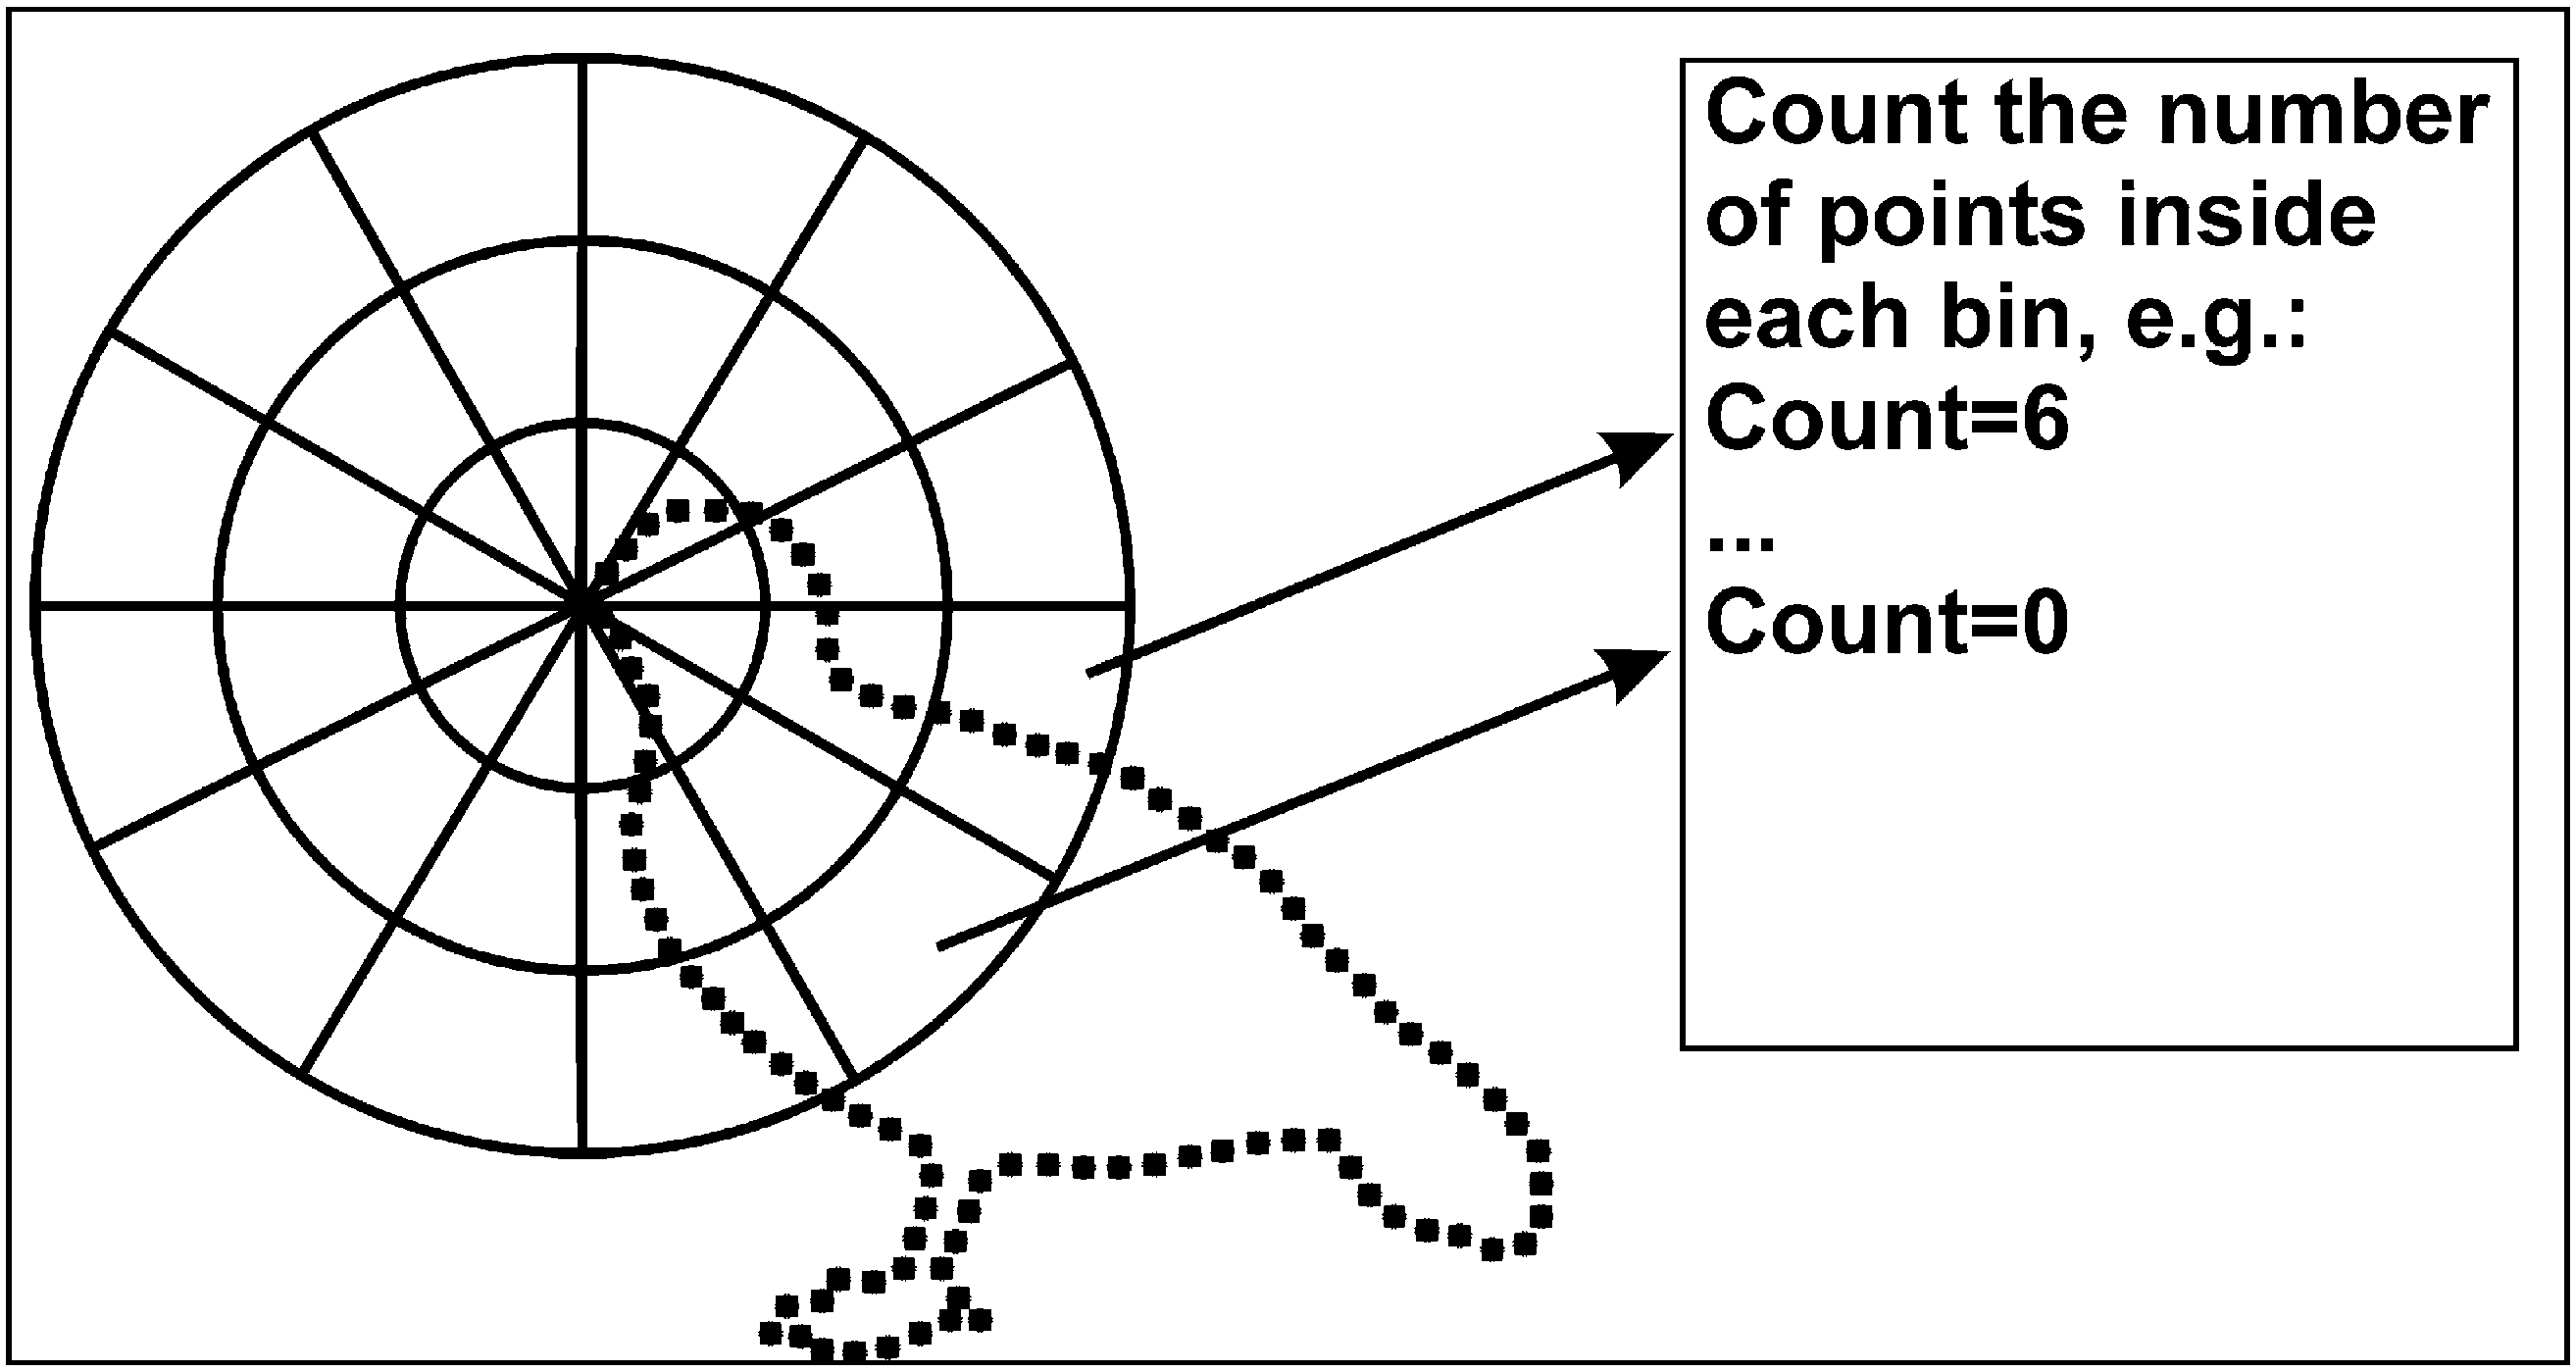
\includegraphics[width=\linewidth]{ext/polarbins.png}
\caption{A scheme of representation of point sets using shape context.
A shape is represented by a discrete set of points sampled regularly along
the contours. For every point, a log-polar histogram—the shape context—is
computed which approximates the distribution of adjacent point locations
relative to the reference point. Image and description taken from \citet{simple}.}
\label{fig:polarbins}
\end{figure}

We can achieve scaling invariance by normalizing all radial distances by the mean distance, and rotation invariance is obtained when searching for the lowest cost among all permutations. According to the paper, this method is also robust against small geometric disturbances.

\section{Matching of shapes using dynamic programming}

A method proposed by \citet{convex} introduces an algorithm which uses dynamic programming combined with high-level features extraction. Similarly to the previous algorithms, the method is based on computation of a distance between the template and the image, but in a different way.

The algorithm requires that the both shape and the template are represented as a sequence of convex and concave line segments, split by inflex points. The idea of the algorithm is to recursively merge segments using two grammar rules $CVC \to C$ and $VCV \to V$, where $V$ denotes concave and $C$ convex segment. Simultaneously, merging cost when the rules are applied is computed using a merging cost function, and the results are stored in the dynamic programming table. The merging cost represents a measure of dissimilarities between the merged segments of the shapes.

Rows and columns of the dynamic programming table represent the inflex points of the shape and the template, respectively. The cost $D(A,B)$ of matching shape $A$ with shape $B$ is defined as:
\[ D(A,B) = min_{T} \{g(i_T,j_T)\}, \]
where $\{g(i_T,j_T)\}$ is a cost of a complete match. The complete match is characterized by a complete path $((i_{0},j_{0}),(i_{1},j_{1}, ..., (i_{T},j_{T}))$, i.e., a path that covers all segments of both shapes. In turn, $\{g(i_T,j_T)\}$ is defined as follows:

\[
g(i_{T},j_{T}) = min(i_w,j_w) \sum_{w=1}^{T} \phi(a(i_{w-1}|i_{w}), b(j_{w-1}|j_{w}))
\]

Expression $\phi(a(i_{w-1}|i_{w}), b(j_{w-1}|j_{w}))$ represents the dissimilarity cost function defined as: 
\begin{align*}
\phi(a(i_{w-1}|i_{w}), b(j_{w-1}|j_{w}))  = \lambda & \textsc{MergingCost}(a(i_{w-1}|i_{w})) \\
+ \lambda & \textsc{MergingCost}(b(j_{w-1}|j_{w})) \\
+ &\textsc{DissimilarityCost}(a(i_{w-1}|i_{w}), b(j_{w-1}|j_{w}))
\end{align*}

The first two terms in represent the cost of merging segments $a(i_{w-1}|i_{w})$ in shape A and segments $b(j_{w-1}|j_{w})$ in shape B, respectively, while the last term is the cost of associating the merged sequence $a(i_{w-1}|i_{w})$ with the merged sequence $b(j_{w-1}|j_{w})$. Each merging should be a recursive application of the grammar rules  $CVC \to C$ and $VCV \to V$.

The lambda value controls merging tendency. With lower value, merging is more encouraged. For shapes with much detail, it is practical to set higher values, otherwise, these details may be lost during merging. 

At the end of the computation, each field $F(i,j)$ of the dynamic table contains the minimal cost of merging the first $i-1$ segments of the shape and $j-1$ segments of the template. The lower the merging cost is, the more are the segments similar. 

Since the algorithm assumes, that first segments of the shape and the template are aligned and match, we may need to run the algorithm for all possible starting points of shape if we don not know the first segment beforehand.

Differently to the previous algorithm, we now require the extraction of high-level features, we need to extract convex and concave segments in correct order. However, we obtain a matching algorithm that is independent of shape translation, scaling and rotation. We can also directly control the invariance to deformations using the lambda parameter.

\section{Neural networks}
Neural networks are mathematical models of computation inspired by a behavior of a biological nervous system \cite{bishop}. They have been successfully used to solve problems in many different areas, including image and pattern recognition. They can be used to solve problems, where we can not easily mathematically describe the solution given the instance of the problem, for reasons of either complexity or lack of existing mathematical model.

\sloppypar Neural networks have several advantages over the previous methods. They do not require feature extraction since they are able to learn it, so we can use pixel values directly. They also have a great ability to generalize, which can be used for the recognition of the shape compositions and embeddings. On the other hand, they have to go through a learning process before they can be used.

\subsection{Neuron}
Artificial neural networks are structures based on the parallel computational model of the biological neural systems. The basic network unit is a neuron (see \cref{fig:neuron}), which is characterized by its input and output connection weights, the activation function and a bias. The artificial neural network is built from a number of connected neurons, usually in a layered structure, and the network learning can be characterized as a process of altering the weights of the connections between neurons and the biases of the neurons. 

\begin{figure}
\centering
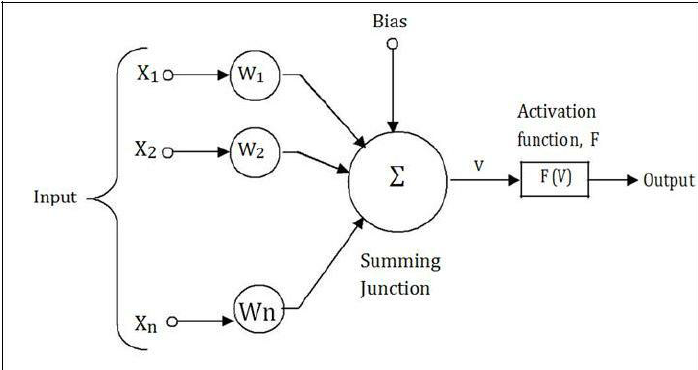
\includegraphics[width=.5\linewidth]{ext/neuron.png}
\label{fig:neuron}
\caption{The model of a neuron unit. Image taken from \citet{neuron}}
\end{figure}

Activation function characterizes the behavior of the neuron. When the values from the input connections are available, the activation function is applied onto the sum of the values and the result is passed further to other neurons. Two common examples of activation functions are the step function and the sigmoid function:

\begin{itemize}
\item $\textsc{Step}(x)=\begin{cases} 1 & (x \geq 0) \\ 0 & (x < 0) \end{cases}$
\item $\textsc{Sigmoid}(x) = \frac{1}{1+e^{-x}} $
\end{itemize}

\subsection{Artificial neural networks}
An artificial neural network is a mathematical model, consisting of a set of neurons interconnected by connections.
More exactly it is a set 
$M  =  (N,C,I,O,w,t)$,  where:
\begin{itemize}
\item $N$  is  a  finite  set  of  neurons.
\item $C \subset N \times N$  is  nonempty  set  of  oriented  connections.
\item $I \subset N$  is  nonempty  set  of  input  neurons.
\item $O \subset N$  is  nonempty  set  of  output  neurons.
\item $w : C \to R$  is  weight  function.
\item $t : N\to R$  bias  function.
\end{itemize}

In practice, multilayer neural networks are commonly used. Multilayer networks are networks, in which the neurons are organized in layers starting with the input layer and ending with the output layer, with hidden layers in between. For each neuron in this structure, its input connections originate only in the previous layer, and its output connections reach only to the following layer.

\subsection{Learning process}
Learning process of an neural network is an optimization problem, where we want to optimize the error function. Error function describes a difference between actual and expected output values for given set of training data. One of the popular error functions is mean square error function:
\[
\textsc{MSE} = \frac{1}{n} \sum_{i=1}^{n} (Y_{i} - \hat{Y}_{i})^2.
\]

Learning process consists of showing inputs to the network and adjusting its connection weights based on the actual and correct output values in order to lower the \textsc{MSE}.

\subsection{Learning algorithms}

\subsubsection{Back-propagation algorithm}
Back-propagation is one of the most popular algorithms for neural networks training, and it serves as a base for many other algorithms.

The algorithm is based on the gradient descent method. In the first step, the input is evaluated and the mean square error of the output is computed. However, a different error function may be used. We can compute the gradient $\frac{\partial E}{\partial w_{ij}}$ for a given training sample using the chain rule
\[
\frac{\partial E}{\partial w_{ij}} = \frac{\partial E}{\partial in_{i}} \frac{\partial in_{i}}{\partial w_{ij}} = 
a_{j}*\frac{\partial E}{\partial in_{i}} = a_{j}*\frac{\partial E}{\partial a_{i}}*\frac{\partial a_{i}}{\partial in_{i}},
\]
where $E$ is the error function, $w_{ij}$ is the weight of the connection between the neurons $i$ and $j$, $in_{i}$ is the weighted sum of the inputs of the neuron $i$ and $a_{i}$ is the output value of the neuron $i$.

If we use the sigmoid activation function denoted $g$, the derivation is:
\begin{equation*}
\frac{dg}{dx}  =  g(x)(1-g(x))
\end{equation*}
which gives us:
\begin{equation*}
\frac{\partial E}{\partial in_{i}} = a_{i}(1-a_{i}) \frac{\partial E}{\partial a_{i}}.
\end{equation*}
We can put the equations together to obtain:
\begin{equation*}
\frac{\partial E}{\partial w_{ij}} = a_{j} a_{i}(1-a_{i}) \frac{\partial E}{\partial a_{i}}
\end{equation*}
There we have two possible cases for the neuron $i$:
\begin{enumerate}
\item [1.] $i$ is an output neuron. Then we get: 
	\[
	\frac{\partial E}{\partial a_{i}} = -(t_{i} - a_{i})
	\]
	where the $t_{i}$ is the expected output for the neuron $i$ for the current input.

\item [2.] $i$ is a hidden neuron. In this case we consider all neurons $k$ that receive input from $i$. Since we are propagating backwards, we know the values $\frac{\partial E}{\partial a_{k}}$ for all $k$. Using chain rule again gives us:
	\[
	\frac{\partial E}{\partial a_{i}} = \sum_{k} \frac{\partial in_{k}}{\partial a_{i}} \frac{\partial E}{\partial in_{k}}
	\]
and from combining the equations we get:
	\[
	\frac{\partial E}{\partial a_{i}} = \sum_{k} w_{ki}a_{k}(1-a_{k}) \frac{\partial E}{\partial a_{k}}
	\]
\end{enumerate}
Now we have defined gradient values $\frac{\partial E}{\partial w_{ij}}$ for all weights in a given neural network.
We can then use the following rule to update the weights:
\[
\Delta^{t} w_{ij} = - \epsilon \frac {\partial E}{\partial w_{ij}} + \alpha \Delta w^{t-1}_{ij}.
\]
$\Delta^{t} w_{ij}$ is the change at time $t$ for the weight $w_{ij}$. The value $\epsilon$ is called the learning rate. If the learning rate is too low, it will take much longer to train the network. If it is too high, the algorithm will cross large section in the search space and will probably oscillate.

In summary, the input is evaluated and the difference between the correct and actual output is computed using error function. The difference is propagated back through the network and weights are updated using the gradient descent method. The whole process is repeated until the desired error value is achieved.

\subsubsection{Quick-prop algorithm}
The quick-prop algorithm is an improved version of the backpropagation. It is based on independent optimization steps for each weight, rather than updating all weights at once. For the update computation, it also requires data from the last iteration, which increases space complexity. The modified $\Delta$ function of the quick-prop algorithm is:
\[
\Delta ^{t} w_{ij} = \Delta^{t-1} w_{ij}*(\frac {\bigtriangledown_{ij} E^{t}} {\bigtriangledown_{ij} E^{t-1} - \bigtriangledown_{ij} E^{t}})
\]
where $\Delta ^{t} w_{ij}$ is the weight delta from $t$-th iteration and $\bigtriangledown_{ij} E^{t}$ denotes partial $w_{ij}$-derivation of error function E in \emph{t} iteration.

\subsection{Advanced structures of neural networks}
There are several advanced techniques in the neural networks field that are commonly used. We describe two of them, the convolution networks and deep neural networks.

\begin{description}
\item [Deep neural networks]
All neural networks with more than two hidden layers can be considered deep neural networks. With the advantage of more layers, deep neural networks can outperform other methods of machine learning. The process of training such network is called \emph{deep learning}. 

More layers allow the network to make more complicated model abstractions over the data. However, there are many challenges to overcome. Deep neural networks have a large number of parameters and training them is demanding on computational power. They are also prone to overfitting, as the added layers of abstraction allow them to find possible unforeseen dependencies in the training data.

\item [Convolutional neural networks]
Convolutional networks can be considered a special case of deep neural networks, because they usually have higher number of layers. They are well suited for pattern recognition directly from the pixels of the image because of their structure of layers with different purposes.
For convolutional networks the convolutional layer is characteristic. This layer is essentially a filter, that performs feature extraction. The filter is composed from neurons that have shared weights, so that the filter performs the same operation on every part of the input. This in turn lowers the number of parameters of the network. Usually, more than one filter is used on the input image, allowing the network to extract different features from the simple ones like edges and corners, to very complex features, such as a house or a tree.
\end{description}

Despite of the performance advantages, we have decided to use the classic feed-forward neural networks with two hidden layers. Because we want to allow the users train the network for their own defined shapes, we need to be able to perform the learning on the user side and offer a simple interface to do so.
This does not correspond well with the advanced neural network structures, which may require certain costly hardware or complicated learning process. Learning of classic neural networks is cheap in comparison, and they can still perform quite well in the recognition tasks.

\subsection{Data preparation for pattern recognition}
Because of their generalization properties, neural network are successfully used in pattern recognition. They are able to approximate an arbitrary mapping between the input values and the output values \cite{bishop}. With this ability, we are not forced to do feature extraction and we can initialize the network with pixel values directly.

It is however recommended to apply several pre-processing transformations that can improve the generalization performance significantly.
\begin{description}
\item [Input normalization]
One of the common forms of pre-processing is input normalization. By applying a linear transformation we can arrange all of the inputs to have zero mean and unit standard deviation over the transformed training set.
In practice, input normalization ensures that the inputs and target outputs stay in unit range, and we can expect that the weights should also be in unit range. We can then initialize the weights with suitable random number. Otherwise, we would have to find a solution, where the weight values differ distinctly.
\item [Training with noise]
Another technique that improves generalization capabilities of the network is training with noise. It involves the addition of a random vector to the input vectors during training. A remark by \citet{bishop} states that:
\begin{quotation} Heuristically, we might expect that the noise will `smear out' each data point and make it difficult for the network to fit individual data points precisely, and hence will reduce over-fitting. In practice, it has been demonstrated that training with noise can indeed lead to improvements in network generalization.
\end{quotation}
\item [Data dimensionality reduction]
Data dimensionality reduction is a pre-processing method that allows the network to have fewer input neurons. It can take the the form of color information removal or pixel averaging, where we group several pixel to one block and use average of each block as an input. By lowering the number of inputs, we lower the number of parameters that the learning process has to optimize.
\item [Feature extraction]
Some of the more complicated techniques use feature extraction as a pre-processing step. Simple geometric primitives extractions are common, such as extraction of lines with their lengths and angles.
\end{description}
